% $Id: conclusion.tex 
% !TEX root = main.tex

%%
\section{\ac{RL} Agents with Adaptive Behavior}
\label{sec:implementation}

This section introduces \adaptiverl, our proposed approach for enabling \ac{RL} agents to dynamically 
adapt their behavior in response to evolving environmental conditions; specifically changes to 
environment goals and changes to agents' actions. Our method allows agents to pursue changing 
objectives throughout their operational lifespan and acquire new capabilities as tasks change over 
time. \adaptiverl is made of three main parts:
\begin{enumerate*}[label=(\arabic*)]
\item monitoring the environment for changes,
\item adapting to new goals, and
\item acquiring new behavior.
\end{enumerate*}
The implementation of our work is publicly available\footnote{Available at: \url{https://github.com/rulas99/rl_uniandes}}.

The conceptual foundation of \adaptiverl aligns with the ideas proposed 
by~\citet{abel2023definitioncontinualreinforcementlearning} for \ac{CRL}, emphasizing continual 
adaptation rather than convergence to a fixed solution. We extend tabular Q-learning by integrating 
adaptive mechanisms that enable agents to dynamically adjust their learning strategies in response 
to detected environmental changes. Similar to the approach described 
by~\citet{norman2024firstexploreexploitmetalearningsolve}, every time a change is detected, be that 
a significant change in the rewards or the introduction of new actions, our agent thoroughly explores 
the environment while retaining information of previously learned policies. The exploration process 
continues until a new policy stabilizes, to then exploit the acquired knowledge. Applying such strategy 
agents can rapidly convergence to new environment configurations, without entirely discarding 
previously learned knowledge.

To enable agents to adapt their behavior to new conditions, we introduce an adaptive mechanisms 
that adjust the agent's learning rate (\lrate{\alpha}) and exploration rate ($\varepsilon$) in conjunction 
with a concept drift detection strategy. By continuously monitoring and responding to changes in the 
environment, agents can autonomously modify their learning process at run time, enabling them 
to learn new behavior to attain their goals, even if these change. This capability positions our approach 
within the class of self-adaptive systems (SAS)~\cite{sasreview}, ensuring continual adaptation and 
resilience in non-stationary contexts.

The key to our approach is given by dynamically adjusting the learning rate (\lrate{\alpha}) based on 
the Temporal Difference (TD) error defined in \fref{eq:td_error}.

\begin{equation} \label{eq:td_error}
    TD_{error} = r_{t+1} + \gamma \cdot \underset{a}{\max} Q(s_{t+1}, a) - Q(s_t, a_t)
\end{equation}

The TD error quantifies the difference between the agent's predicted reward and the actual reward 
received. The dynamic learning rate (\lrate{\alpha^*}) is then adjusted based on the TD error following  
\fref{eq:dynamic_learning_rate}.

\begin{equation}
    \label{eq:dynamic_learning_rate}
    \alpha^* = \alpha + (\alpha_{\max}-\alpha) \cdot \frac{1}{1 + e^{-(|TD_{error}|-k)}}
\end{equation}

In the equation, \lrate{\alpha} corresponds to the base learning rate (e.g., 0.1), and $\alpha_{\max}$ is its upper bound (\eg 0.99). The parameter $k$ controls the sensitivity of the learning rate to the TD error, with higher values resulting in reduced sensitivity; thus, $k$ must be carefully tuned according to the specific characteristics of the environment and learning context. High TD errors induce a larger learning rate, enabling faster updates during exploration, whereas lower TD errors yield a more stable and conservative learning process during exploitation phases. \fref{fig:alpha} illustrates the behavior of the dynamic learning rate (\lrate{\alpha^*}) in \fref{sec:experiments} presenting the non-stationary Gridworld experiments. 

\begin{figure*}
    \centering
    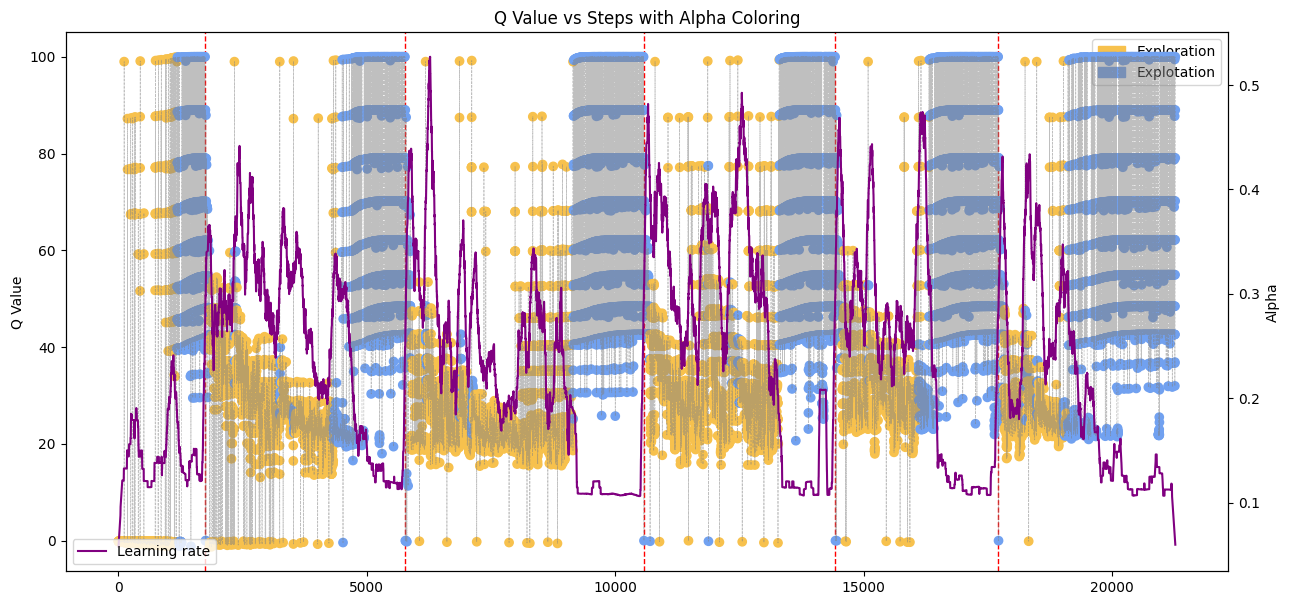
\includegraphics[width=\textwidth]{figures/alpha.png}
    \caption{\adaptiverl's adaptive behavior of the dynamic learning rate ($\alpha^*$) in Non-Stationary Gridworld experiments. Notice how $\alpha^*$ increases during exploration phases (when the TD error is high) and decreases during exploitation phases (when the TD error is low), enabling rapid convergence during exploration and stable learning during exploitation.}
    \label{fig:alpha}
\end{figure*}

%%%%
\subsection{Environment monitoring and drift detection}

The first step for agents to adapt their behavior to an evolving environment is to continuously monitor 
the environment. \ac{RL} environment monitoring is intrinsic through the interaction with the 
environment, as agents continuously observed rewards after each action execution. To detect 
changes in the environment, \ie drift, we implement the 
PH-test~\cite{mignon2017adaptive,networkdynamicrl}. The PH-test calculates the cumulative 
difference between observed rewards and the running mean reward, incorporating a sensitivity 
parameter ($\delta$). A concept drift (environmental change) is flagged when the cumulative 
difference surpasses a predefined threshold. Selecting an appropriate threshold value is crucial, as it 
determines the sensitivity of drift detection. Higher thresholds result in more conservative detection, 
while lower thresholds increase sensitivity to changes, this value must be selected based on the 
magnitude order of rewards and posible changes over them.

Building on the concept of drift detection, and following the ideas of~\citet{mignon2017adaptive}, we 
adaptively increase the exploration rate ($\varepsilon$) whenever the PH-test detects a concept drift. 
This approach promotes exploration immediately following environmental changes, enabling the agent 
to acquire new knowledge by temporarily adopting an exploration-focused policy. To ensure adequate 
exploration, the agent maintains an elevated exploration rate until rewards stabilize (\ie the cumulative 
difference is below the threshold, and  no further drifts are detected). Once stable, the exploration rate 
$\varepsilon$ uses a decay policy, leading the agent to exploit its behavior.

This adaptive drift detection mechanism ensures the agent maintains an effective balance between 
exploring new environment dynamics and leveraging previously acquired knowledge. It is crucial to 
ensure a high exploration rate after concept drift is detected consistently, so the agent can learn a 
new policy (\ie behavior) without forgetting previously acquired knowledge. \fref{fig:dynamic-eps}, 
shows the behavior of the dynamic exploration rate ($\varepsilon^*$) in our non-stationary Gridworld 
running example.

\begin{figure*}
    \centering
    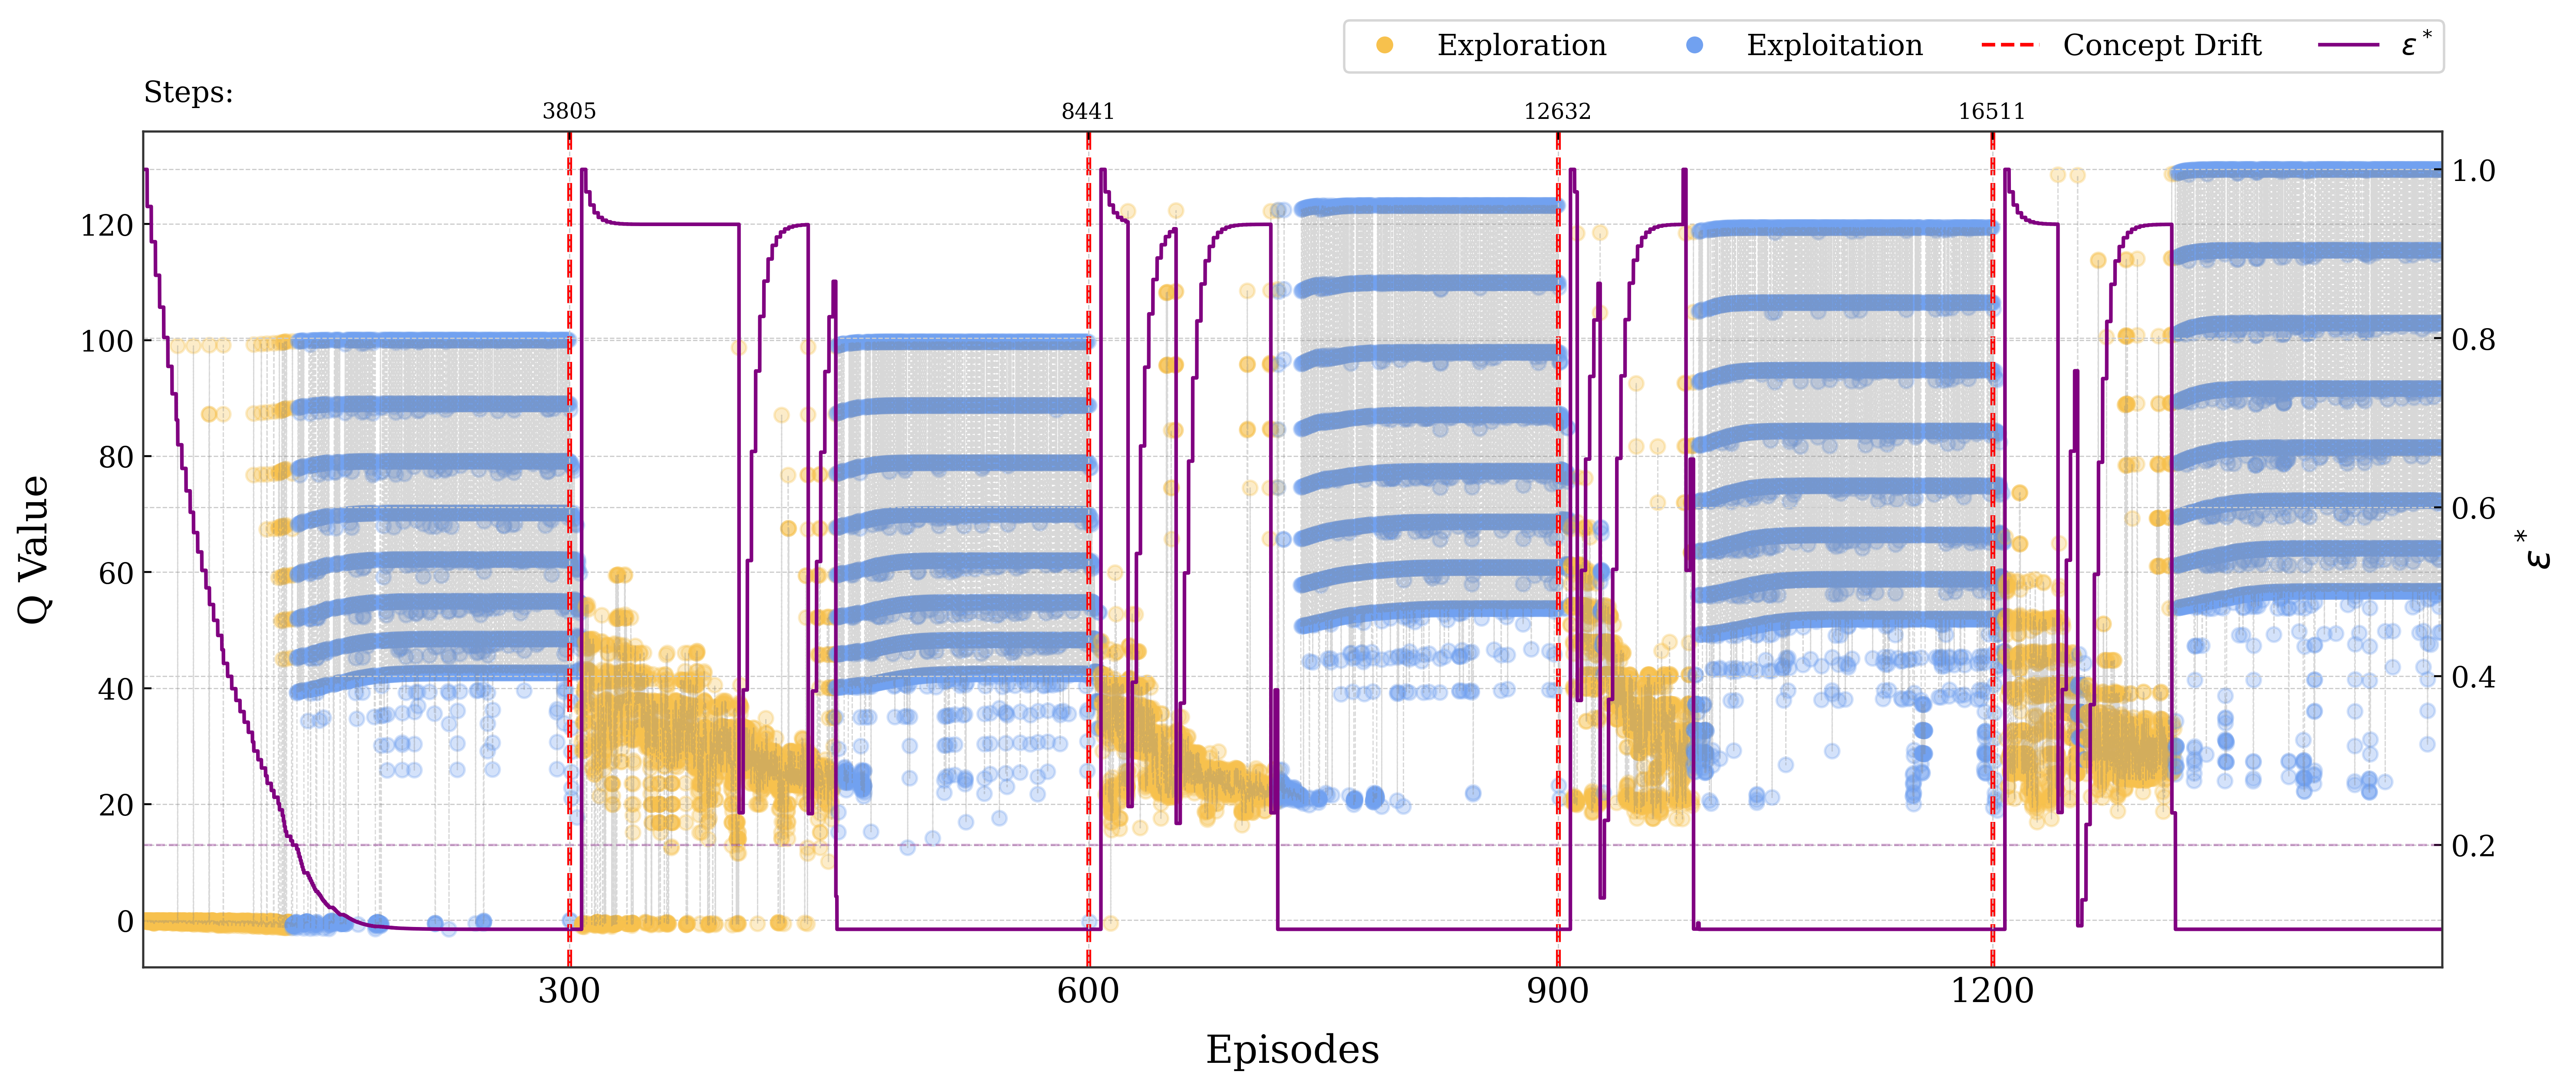
\includegraphics[width=\textwidth]{figures/eps}
    \caption{\adaptiverl's adaptive behavior of the dynamic exploration rate ($\varepsilon^*$) in Non-Stationary Gridworld experiments. Observe how $\varepsilon^*$ increases whenever a concept drift is detected by the PH-test and remains elevated until the agent consistently achieves the expected rewards (i.e., no further drift and stable rewards). Once stability is reached, $\varepsilon^*$ decays toward its minimum value, allowing the agent to exploit the acquired knowledge.}
    \label{fig:dynamic-eps}
\end{figure*}

%%%%
\subsection{Agent Adaptation to Changing Goals}
\label{sec:experiments}

To evaluate \adaptiverl's ability to adapt to environmental changes induced by a non-stationary reward function, and to compare its performance against traditional Q-learning, Gridworld. 

We compare two agents over 1,000 independent runs:  
\begin{itemize}
  \item A \emph{Standard Q-learning} agent, with fixed learning rate $\alpha=0.1$ and a fixed exponential decay for the exploration rate.
  \item A \emph{\adaptiverl} agent, employing the adaptive learning-rate and exploration-rate mechanisms described in above.
\end{itemize}
We measure (1) the number of episodes required to re-converge after each reward change, and (2) the total number of steps across all 1,500 episodes. \fref{tab:multi} reports the mean and standard deviation of the steps-to-goal for each drift, as well as the overall steps.  

\begin{table*}
    \centering
    \caption{Performance of each agent over 1,000 runs: average number of steps $\pm$ relative standard deviation (as a percentage of the mean) to reach the goal after each drift, and total steps for all 1,500 episodes (fewer steps indicate better performance).}
    \resizebox{1.01\columnwidth}{!}{
\begin{tabular}{l | c | c | c | c | c }
\toprule
\textbf{Agent} & \textbf{1st Change} & \textbf{2nd Change} & \textbf{3rd Change} & \textbf{4th Change} & \textbf{Total Steps} \\
\midrule
\adaptiverl & 135.81 $\pm$ 12.64 (9.31\%) & 475.17 $\pm$ 27.54 (5.80\%) & 767.81 $\pm$ 24.05 (3.13\%) & 1069.74 $\pm$ 26.25 (2.45\%) & 23292.07 $\pm$ 1474.13 (6.33\%) \\
Q-Learning  & 256.40 $\pm$ 11.15 (4.35\%) & -- & -- & -- & 40683.74 $\pm$ 539.44 (1.33\%) \\
\bottomrule
\end{tabular}
}

    \label{tab:multi}
\end{table*}

\adaptiverl outperforms the standard Q-learning agent on every metric. Figures~\ref{fig:alpha} and~\ref{fig:dynamic-eps} show how \adaptiverl's adaptive mechanisms enable rapid re-learning of the new goal location without erasing knowledge of previous configurations. This behavior addresses the challenge of overlapping contradictory subtasks~\cite{Bagus2022}, where identical state-action pairs may yield different rewards.

By contrast, the standard Q-learning agent converges reliably only to the first goal configuration. Figure~\ref{fig:static-eps} depicts its exploration rate decay: after each drift, the agent continues to exploit the old policy for an extended period, effectively “forgetting” previous knowledge before it begins learning the new goal location.

\begin{figure*}
    \centering
    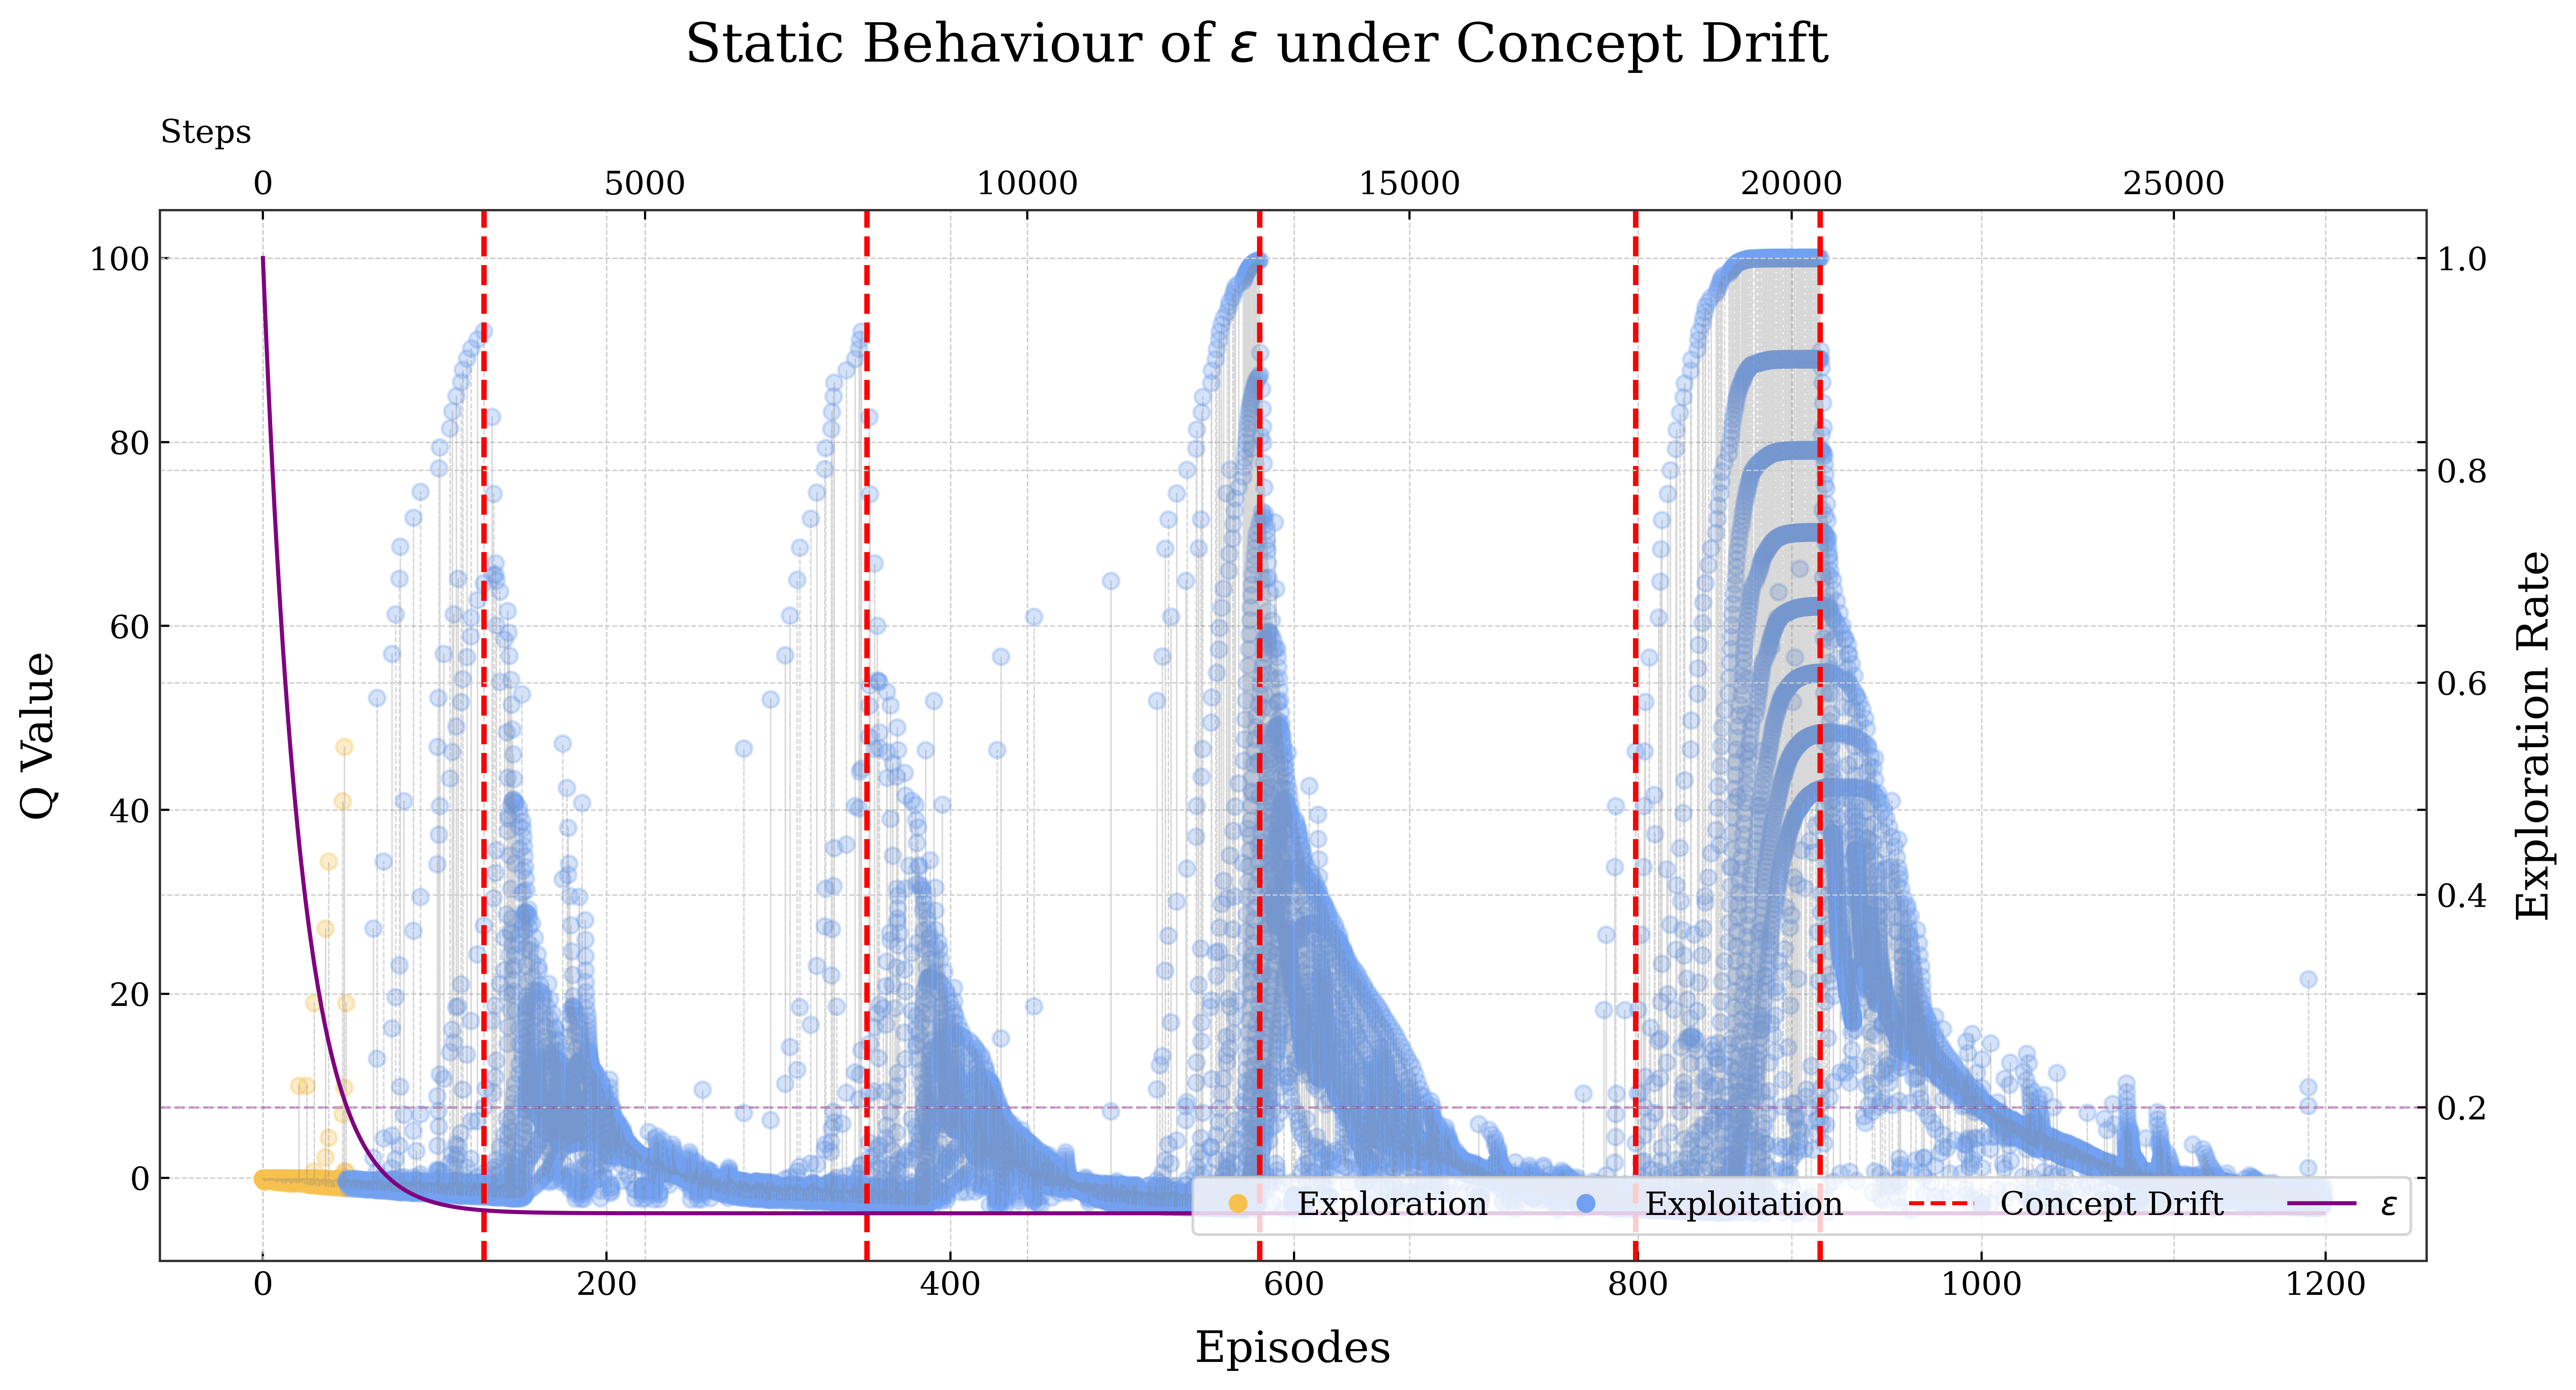
\includegraphics[width=\textwidth]{figures/trad_eps.png}
    \caption{Behavior of the static exploration rate decay ($\varepsilon$) under traditional Q-learning: the agent fails to adapt to any subsequent goal relocation, exhibiting prolonged exploitation of the obsolete policy.}
    \label{fig:static-eps}
\end{figure*}

These results demonstrate that \adaptiverl consistently outperforms standard Q-learning in adapting to changing goals and acquiring new policies without forgetting previously learned knowledge. As shown in Figure~\ref{fig:q-value-comp}, after 1,500 episodes, \adaptiverl maintains high Q-values for all previous goal configurations, whereas traditional Q-learning must overwrite its Q-values each time the goal relocates. Notably, \adaptiverl preserves prior knowledge by promoting exploration for a sufficient period after each detected drift and by scaling updates according to the TD-error magnitude. This approach not only prevents catastrophic forgetting but also enables the agent to handle both contradictory and non-contradictory overlapping subtasks---such as when goals are randomly sampled in nearby regions rather than at the exact same cell\footnote{Animated simulations of these and other scenarios are available at: \url{https://github.com/rulas99/rl_uniandes/tree/main/simulations}}.

While \adaptiverl introduces modest overhead due to drift detection and adaptive updates, its overall 
run-time is actually lower. Using our experimental setting $1,000$ runs take approximately 5
minutes for \adaptiverl, while it takes around 8 minutes to complete all runs with the baseline Q-learning implementation. This efficiency gain results directly from the reduced number of steps needed to reach the goal after each drift. Specifically, \adaptiverl converges in significantly fewer steps than the standard agent---requiring about 1.9x fewer iterations after the first drift and 1.7x fewer over the full 1,500 episodes---highlighting the practical advantages of our adaptive mechanisms in dynamic environments.

\begin{figure*}
    \centering
    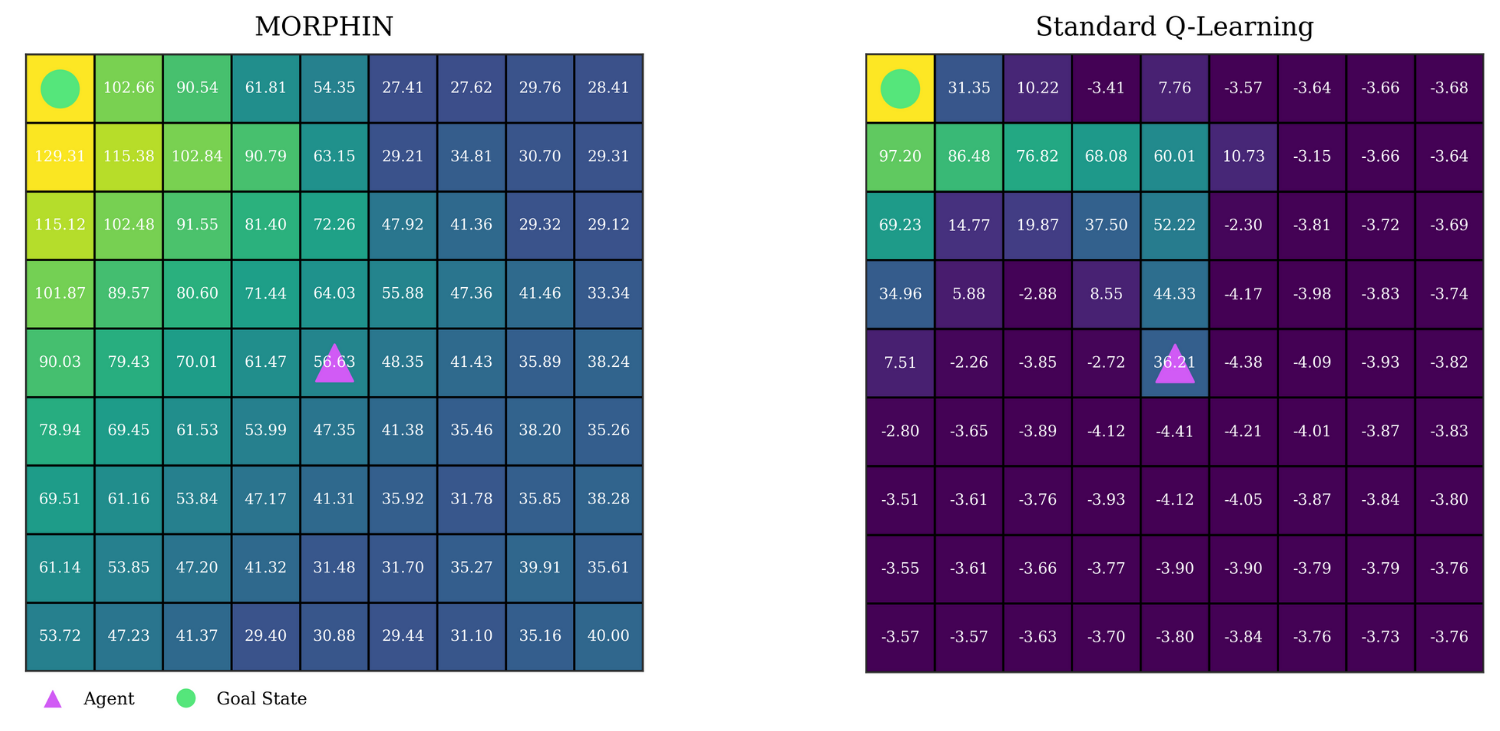
\includegraphics[width=\textwidth]{figures/q_map_comp}
    \caption{Comparison of Q-value heatmaps after 1,500 episodes in a Non-Stationary Reward Environment: (left) \adaptiverl preserves high Q-values across alternating goal configurations; (right) Standard Q-learning must overwrite past knowledge to learn each new goal.}
    \label{fig:q-value-comp}
\end{figure*}

%%%%
\subsection{Acquisition of new actions}
In the next Section~\ref{sec:validation}, we present a real-world use case for traffic light control, where the agent is provided with a new set of actions following concept drift detection. This enables the agent to efficiently learn how to utilize the new actions and optimize traffic flow by adapting its policy to varying congestion levels. The agent can acquire new capabilities without forgetting previously learned behaviors, maintaining adaptability to changing environmental conditions.

These adaptive mechanisms equip the agent to effectively manage learning under varying and unpredictable conditions, enabling continuous adaptation and efficient knowledge transfer between different environmental states. The concept drift detection method with the dynamic exploration rate allows the agent to rapidly respond to new information without discarding previously learned knowledge, achieving a greater resilience and performance stability over its lifespan. 


\endinput

